%template1.tex
%The following LaTeX source file represents the simplest kind of slide presentation; no overlays, no included graphics. Substitute your favorite style for ``pascal''. To create the PDF file template1.pdf, (1) be sure to use the prosper class, then (2) execute the command latex template1.tex, and (3) the command dvipdf template1.dvi.

%%%%%%%%%%%%%%%%%%%%%%%%%%%%%%% template1.tex %%%%%%%%%%%%%%%%%%%%%%%%%%%%%%%%%%%
\documentclass[a4paper,blends,pdf,colorBG,slideColor]{prosper}
% definitions for slides for CSC544
% Lutz Hamel, (c) 2007

\hypersetup{pdfpagemode=FullScreen}

\usepackage{amssymb}
\usepackage{latexsym}
\usepackage{amsmath}
%\usepackage[usenames]{color}
\usepackage{xypic}


\newcommand{\term}[1]{\ensuremath{\mbox{\bf #1}}}
\newcommand{\nonterm}[1]{\ensuremath{\mbox{#1}}}
\newcommand{\ifstmt}[3]{\ensuremath{{\bf if}\; {#1}\;{\bf then}\;{#2}\;{\bf else}\;{#3}\;\term{end}}}
\newcommand{\whilestmt}[2]{\ensuremath{{\bf while}\; {#1}\;{\bf do}\;{#2}\; \term{end}}}
\newcommand{\funcstmt}[3]{\ensuremath{{\bf fun}\; {#1}\; {\bf is}\; {#2} \; {\bf return}\; {#3}}}
\newcommand{\syntaxset}[1]{\ensuremath{\mbox{\bf #1}}}
\newcommand{\orbar}{\;|\;}
\newcommand{\bs}[1]{\begin{slide}{#1}\ptsize{8}}
\newcommand{\es}{\end{slide}}
\newcommand{\co}{\,\colon\;}
\newcommand{\pair}[2]{\ensuremath{\langle {#1}, {#2} \rangle}}
\newcommand{\encode}[1]{\ensuremath{\langle {#1} \rangle}}
\newcommand{\mytab}{\makebox[.15in]{}}
%\newcommand{\abs}[1]{{\mid{#1}\mid}}
\newcommand{\abs}[1]{{|{#1}|}}
\newcommand{\ol}[1]{\overline{#1}}

\newcommand{\qaccept}{\ensuremath{q_{\mbox{\tiny accept}}}}
\newcommand{\qreject}{\ensuremath{q_{\mbox{\tiny reject}}}}
\newcommand{\accept}{{\em accept}}
\newcommand{\reject}{{\em reject}}

\newcommand{\machine}[1]{
	\begin{quote}
	{#1}
	\end{quote}
	}

\newcommand{\fdef}[1]{
	\begin{center}
	\fbox{
	\begin{minipage}{3.5in}
	{\bf Definition:}
	{#1}
	\end{minipage}
	}
	\end{center}
	}

\newcommand{\ftheorem}[1]{
	\begin{center}
	\fbox{
	\begin{minipage}{3.5in}
	{\bf Theorem:}
	{#1}
	\end{minipage}
	}
	\end{center}
	}

\newcommand{\flemma}[1]{
	\begin{center}
	\fbox{
	\begin{minipage}{3.5in}
	{\bf Lemma:}
	{#1}
	\end{minipage}
	}
	\end{center}
	}


\newcommand{\fframe}[1]{
	\begin{center}
	\fbox{
	\begin{minipage}{3.5in}
	{#1}
	\end{minipage}
	}
	\end{center}
	}

\newcommand{\nframe}[1]{
	\begin{center}
	\begin{minipage}{3.5in}
	{#1}
	\end{minipage}
	\end{center}
	}

\begin{document}
\bs{Welcome - CSC 544}
\begin{center}
	{\LARGE\em Theory of Computation}\\

	Dr. Lutz Hamel\\
	hamel@cs.uri.edu\\
	Tyler Hall, Rm 251\\
	\vspace{.3in}

    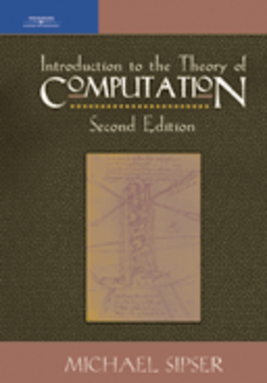
\includegraphics[height=35mm]{images/sipser-book.ps}
\end{center}

\es

\bs{Optional Reference Material}
{\small
Other books you might find useful/interesting to consult:
\begin{itemize}
\item {\em The Annotated Turing: A Guided Tour Through Alan Turing's Historic Paper on Computability and the Turing Machine},  Charles Petzold, Wiley,  2008.
\item {\em Alan Turing: Life and Legacy of a Great Thinker}, Christof Teuscher (Editor), Springer, 2006.
\item {\em The Universal Computer: The Road from Leibniz to Turing}, Martin Davis, W. W. Norton \& Company, 2000.
\end{itemize}
}
\es

\bs{The {\em What} and the {\em Why}}
\begin{description}
\item[What:] The {\em Theory of Computation} is the formal (mathematical) investigation of models of computation.

\item[Why:] We investigate models of computation in order to understand the nature of computation without having to worry about specific hardware.  

However, if the models reflect the major characteristics 
of the hardware implementation, then the laws of computation discovered in the models are also 
applicable to the actual hardware!  Thus, the theoretical results are directly applicable to software design.

The nature of computing does not only involve limits of computability, but also problem complexity.  We could be faced
with a perfectly computable function (whatever that means at this point) but the time complexity of this function is such that the computation would never complete in a reasonable amount
of time  (whatever that means at this point).

\end{description}
\es

\bs{Models of Computation}
\begin{enumerate}
\item Finite Automata
\item Turing Machines
\item $\lambda$-Calculus -- invented by Alonzo Church to investigate the nature of computation
\item Recursive Functions -- a term coined by R\'{o}zsa P\'{e}ter a Hungarian mathematician and used by Kurt G\"{o}del in some of his famous proofs
\item String Rewriting Systems -- also called semi-Thue systems after Axel Thue a Norwegian mathematician
\end{enumerate}

It is interesting to note that
\begin{enumerate}
\item all models of computation except the first one were invented separately by logicians
in the early 1900's and have been shown to be equivalent, they each can simulate the other 
\item Turing machines can simulate finite automata in a straightforward manner (but not vice-versa)
\end{enumerate}
\es


\bs{Models of Computation}
In this course we will start with a brief overview of results in automata theory and we will then
continue to study the majority of computability and complexity theoretical results in the context
of Turing machines.

We will also show the equivalence between the various models.
\es


\bs{Course Road Map}
\begin{center}
    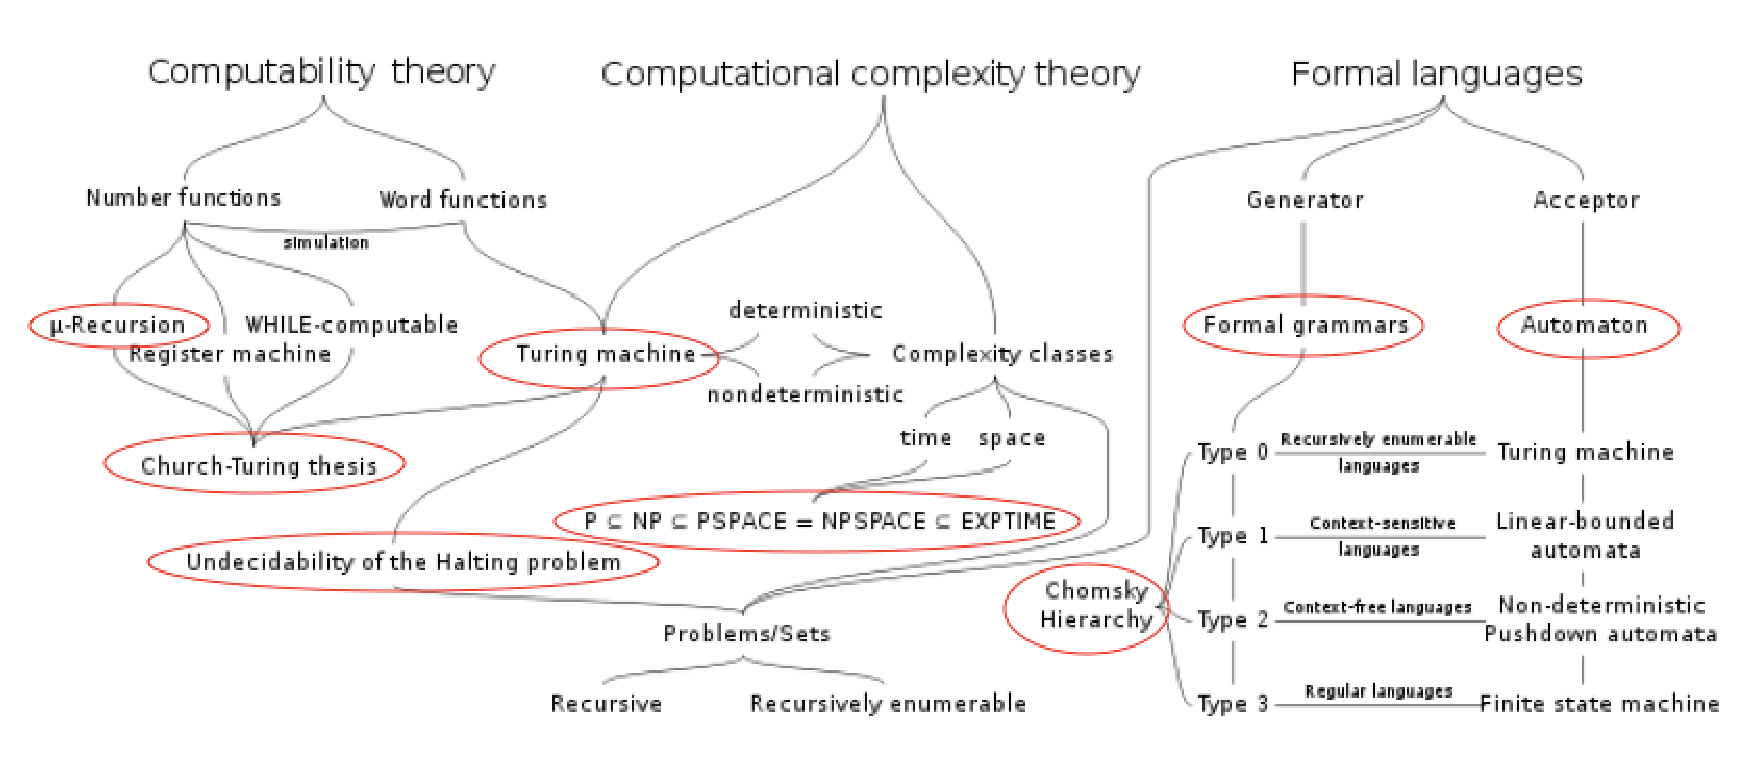
\includegraphics[height=45mm]{images/course-road-map-00.eps}
\end{center}

\es

\bs{\large Limits of Computer Science - The Halting Problem}
Every discipline has its limits.  Consider:
\begin{description}
\item[Physics - The Perpetual Motion Machine] - construct a machine that once set in motion
will produce useful work indefinitely without consuming any energy -- Impossible, violates
the second law of thermodynamics -- entropy alway increases.
\item[Mathematics - Squaring of the Circle] - with just a compass and a straightedge construct
a square with the same area as a given circle -- Impossible, given that the area of a circle is $r^2 \pi$
we need to construct a square with sides $r \sqrt{\pi}$, however, $\pi$ is a transcendental  number
and therefore not constructable.
\item[Computer Science - The Halting Problem] - write a program that decides, given {\bf any program}, whether
that program will halt for {\bf all inputs} -- Impossible, such a general program cannot be constructed!
\end{description}

\es


\bs{Fundamental Concepts}

\begin{description}
\item[Algorithm] - What does it mean to ``compute" and exactly ``what can be computed"?
\item[Decidability] - Which problems can be solved using algorithms and which cannot?
\item[Complexity] - How much time and space does a particular problem solution require?
\item[Complexity Theory] - Can we organize problems according to the complexities?
\end{description}
\es

\bs{Mathematical Discipline}
The theory of computation is ultimately a mathematical discipline.  We rely on {\em proofs} to investigate
truths and consequences of our model choices.

A proof is a {\em logical argument} that establishes the truth of a statement beyond any doubt.  Here are
common terms associated with proofs:

\begin{description}
\item[Statement:] a sentence that is either true or false.
\item[Axiom:] a statement that is assumed to be universally true.
\item[Assumption:] a statement that is assumed to be true for the current proof at hand.
\item[Definition:] an unambiguous statement of the precise meaning of a word, symbol, phrase, or
concept.
\item[Theorem:] a universal statement whose truth can be established using a chain of logical reasoning on the basis of certain assumptions that are explicitly given or implicit in the statement.  Such a construction
is called a {\em proof of a theorem}.
\end{description}
\es

\bs{Mathematical Discipline}

\begin{description}
\item[Lemma:] a statement in the context of the current proof whose truth can be established using a chain of logical reasoning (see theorem).  A non-universal/auxiliary theorem to be used in the proof of another theorem.

\item[Corollary:] a theorem that follows {\em logically and easily} from another theorem already proved.
\end{description}

\es


\bs{The Structure of a Proof}
Lemmas with their proofs.

Statement of the Theorem.

Proof of the theorem:
\begin{itemize}
\item axioms
\item assumptions
\item logical  reasoning steps
\item conclusion
\end{itemize}
\es


\bs{Proof Test Drive}
{\bf Definition:} $q \in A \cap B$ iff $q\in A$ and $q \in B$.

{\bf Definition:} $q \in A \cup B$ iff $q\in A$ or $q\in B$. 

{\bf Theorem:} Given two sets $A$ and $B$, then $\overline{A \cup B} = \overline{A} \cap \overline{B}$.

{\bf Proof:} In order to show that the equivalence $\overline{A \cup B} = \overline{A} \cap \overline{B}$ holds, we need to show that $\overline{A \cup B} \subseteq \overline{A} \cap \overline{B}$ and
$\overline{A} \cap \overline{B} \subseteq \overline{A \cup B}$ holds.

(1) $\overline{A \cup B} \subseteq \overline{A} \cap \overline{B}$. Let some $x \in \overline{A \cup B} $,
this implies that $x\not\in A \cup B$.  Therefore, $x\not\in A$ and $x\not\in B$.  From this it follows
that $x\in \overline{A}$ and $x\in\overline{B}$.  Given the definition of intersection of sets, it follows
that $x \in \overline{A} \cap \overline{B}$.

(2) $\overline{A} \cap \overline{B} \subseteq \overline{A \cup B}$. Let some $x \in \overline{A} \cap \overline{B}$, this implies $x \in \overline{A}$ and $x \in \overline{B}$ or $x\not\in A$ and $x\not\in B$.
It follows that $x \not\in A\cup B$ or expressed as the complement $x \in \overline{A \cup B}$.

This concludes the proof. $\Box$.
\es

\bs{Types of Proofs}
\begin{description}
\item[Proof by Construction:] Many theorems posit that certain objects exist.  One way
to prove the existence of these objects is to construct them.

\item[Direct Proof:] A straight forward application of the modus ponens, 
{\scriptsize
\begin{quote}
Given, $A$ implies $B$.\\
Assume $A$.\\
Show that $B$ holds.
\end{quote}
}

\item[Proof by Contradiction:] (also called indirect proof),
{\scriptsize
\begin{quote}
Assume $A$.\\
Assume $\neg B$.\\
Show that $\neg B$ implies $\neg A$ (contradiction!)\\
Therefore, $B$ has to hold.
\end{quote}
}

\item[Proof by Induction:] Example, assuming a well-founded relation on some domain, such as the
successor relation $+1$ on the positive integers {\cal I}, and given some predicate  $P$,
then we can show that $\forall i \in {\cal I}.P(i)$ iff $P(1)$ and $P(n+1)$ assuming that
$P(n)$ holds.
\end{description}
\es
\end{document}
%%%%%%%%%%%%%%%%%%%%%%%%%%% end of template1.tex %%%%%%%%%%%%%%%%%%%%%%%%%%%%%%%%

